% Based on the official cvpr-org/author-kit, commit 291758547e923160eb4d37079b7b9f0dfce82355.
% The latest released kit at drafting time is CVPR 2026; update the kit when CVPR 2027 releases one.
\documentclass[10pt,twocolumn,letterpaper]{article}
\usepackage[review]{cvpr}
%% This file contains a number of tweaks that are typically applied to the main document.
%% They are not enabled by default, but can be enabled by uncommenting the relevant lines.


%%
%% Official support for 2-column teaser figure
%%
\usepackage{cuted} %< for strip environment

%%
%% For auto-referencing of figures (see fig/teaser.tex and \label{} therein) 
%%
\usepackage{currfile} %< for \currfilebase macro

%%
%% caption and (global) spacing overrides
%%
\usepackage{caption} %< for "\captionof" commands (teaser)
% \setlength{\abovecaptionskip}{.5em} % space above caption
% \setlength{\belowcaptionskip}{1em} % space below caption

%%
%% Inline annotations; for predefined colors, refer to "dvipsnames" in the xcolor package:
%% https://tinyurl.com/overleaf-colors
%%
\newcommand{\red}[1]{{\color{red}#1}}
\newcommand{\todo}[1]{{\color{red}#1}}
\newcommand{\TODO}[1]{\textbf{\color{red}[TODO: #1]}}
%%
%% Disable for camera ready / submission by uncommenting these lines:
%%
% \renewcommand{\TODO}[1]{}
% \renewcommand{\todo}[1]{#1}

%%
%% Work harder in optimizing text layout. Typically shrinks text by 1/6 of page, enable
%% it at the very end of the writing process, when you are just above the page limit.
%%
% \usepackage{microtype}

%%
%% Fine-tune paragraph spacing.
%%
% \renewcommand{\paragraph}[1]{\vspace{.5em}\noindent\textbf{#1.}}

%%
%% Globally adjusts space between figure and caption.
%%
% \setlength{\abovecaptionskip}{.5em}

%%
%% Allows "the use of \paper to refer to the project name"
%% with automatic management of space at the end of the word.
%%
% \usepackage{xspace}
% \newcommand{\paper}{ProjectName\xspace}

%%
%% Commonly used math definitions.
%%
% \DeclareMathOperator*{\argmin}{arg\,min}
% \DeclareMathOperator*{\argmax}{arg\,max}

%%
%% Tighten underline.
%%
% \usepackage{soul}
% \setuldepth{foobar}

%%
%% Reconfigure paragraph (tweaks spacing)
%%

\usepackage{amsmath,amssymb,booktabs,graphicx,multirow}
\definecolor{cvprblue}{rgb}{0.21,0.49,0.74}
\usepackage[pagebackref,breaklinks,colorlinks,allcolors=cvprblue]{hyperref}
\def\paperID{*****}
\def\confName{CVPR}
\def\confYear{2027}
\title{EventTrace: Verifying Ordered Semantic Events for Reinforcement Fine-Tuning of Vision-Language Navigation}
\author{Anonymous CVPR Submission}

\begin{document}
\maketitle

\begin{abstract}
Reinforcement fine-tuning of vision-language navigation (VLN) policies commonly relies on destination success or similarity to a reference route. These signals may leave an instruction's intermediate requirements unresolved: reaching the endpoint does not establish that the agent entered the requested room or passed the specified landmark. We study an online reward that represents an instruction as an ordered list of semantic events and verifies each event against the observations before and after an executed action. A frozen vision-language model supplies a three-way verdict (complete, incomplete, uncertain), while motion and stopping checks rule out visually plausible but unexecuted events. An event is rewarded at most once and the total process reward is bounded below a success bonus. We implement this reward in a multi-turn ActiveVLN/GRPO training pipeline and report a controlled feasibility experiment on eight R2R training episodes. Across two optimization steps per arm, event and destination-only training each attain 13 successes in 16 sampled rollouts; the event arm records 23 confirmed event completions and 33 uncertain turn verdicts. Identical first-step action sequences show that the reward difference reaches the optimizer. On a fixed exploratory 16-episode val-unseen subset, the SFT, destination-only, and event checkpoints each succeed in 6 episodes. The study demonstrates reward integration but does not demonstrate a navigation gain.
\end{abstract}

\section{Introduction}
Vision-language navigation asks an embodied agent to follow a natural-language route through visual observations. The Room-to-Room (R2R) task introduced instruction-guided navigation in real indoor environments~\cite{anderson2018r2r}; VLN-CE moves this task into continuous control~\cite{krantz2020vlnce}. Success rate (SR) and success weighted by path length (SPL) capture destination attainment, yet a successful stop can coexist with skipped intermediate instructions. Instruction fidelity work made this gap explicit~\cite{jain2019cls}.

Recent reinforcement fine-tuning (RFT) approaches give visual-language policies online or trajectory-level feedback. ActiveVLN performs multi-turn exploration with group-relative policy optimization (GRPO)~\cite{zhang2025activevln,shao2024deepseekmath}. VLN-R1 uses time-decayed action rewards~\cite{qi2025vlnr1}; Nav-R1 combines format, understanding, and navigation rewards~\cite{liu2025navr1}; SeeNav-Agent proposes step-level verifiable process rewards in another navigation benchmark~\cite{wang2025seenav}. Our question is narrower: can a navigation instruction's ordered, physical events provide a bounded reward during \emph{closed-loop} R2R-CE rollouts, without matching the policy's actions to a reference path?

We introduce \emph{EventTrace}, a modular reward on top of an existing multi-turn policy. The reward uses a short event list, a frozen visual verifier with an abstention state, deterministic checks of motion or stopping, and a once-only order-preserving tracker. The actor sees only the original egocentric observations and instruction; simulator displacement is available only to the reward. Figure~\ref{fig:example} illustrates the distinction between seeing a bathroom and actually entering it.

The present manuscript reports a feasibility pilot and a small held-out probe rather than a claim of improved navigation. We make the implementation, measured counts, and limitations explicit so that a larger study can test the central hypothesis without confusing a changed reward scale with improved SR.

\begin{figure}[t]
\centering
\begin{tabular}{@{}cc@{}}
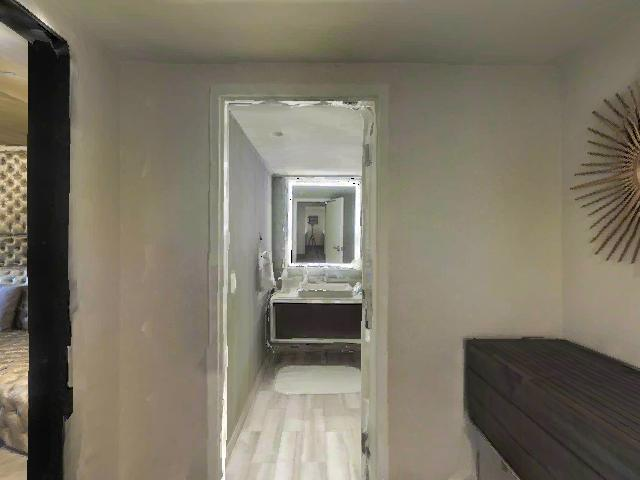
\includegraphics[width=.46\linewidth]{figures/bathroom_before.jpg} &

\includegraphics[width=.46\linewidth]{figures/bathroom_after.jpg}\\
(a) Doorway view & (b) Interior view
\end{tabular}
\caption{Real simulator frames from a diagnostic replay of R2R training episode 2889. Visibility alone does not complete the event ``enter bathroom.'' The verifier uses before/after views and executed motion; the ordered tracker later checks ``stop near sink.'' These frames illustrate the mechanism and are not an independent accuracy test.}
\label{fig:example}
\end{figure}

\section{Related Work}
\paragraph{Path and instruction fidelity.} SR and SPL reward the destination and efficiency, whereas nDTW and coverage weighted by length score (CLS) compare trajectories with a reference route~\cite{ilharco2019ndtw,jain2019cls}. Reference trajectories can be useful supervision but do not directly answer whether a distinct visual event actually occurred when multiple valid routes exist. Our reward targets event completion during execution; route metrics remain complementary evaluation measures.

\paragraph{RL for VLN.} ActiveVLN is our implementation base because its environment can return feedback after each multi-action turn~\cite{zhang2025activevln}. VLN-R1 and Nav-R1 show other ways to shape VLN rewards~\cite{qi2025vlnr1,liu2025navr1}. SeeNav-Agent is especially relevant in its emphasis on step-level verification~\cite{wang2025seenav}. EventTrace differs in its ordered event state, explicit uncertainty outcome, and physical gates against rewarding a landmark seen without the requested transition. Our pilot still applies GRPO to \emph{trajectory-level} returns; it does not claim SeeNav-Agent-style step-level credit assignment.

\section{Method}
\subsection{Task and event representation}
An instruction $x$ yields a list $E(x)=(e_1,\ldots,e_K)$, where $e_k$ contains a verb type, target phrase, and source span. Supported pilot events include \texttt{enter}, \texttt{pass}, \texttt{descend}, and \texttt{stop\_near}. We first generate candidate events using a frozen vision-language model (VLM), check the event verb and target against the instruction, and curate the eight lists used in the pilot. The measured pilot therefore tests reward integration given curated events; it does not validate automatic instruction parsing.

The parser is constrained to at most three events and the source span must appear in the original instruction. In the curated pilot, each of the eight episodes contains a stopping event; there are also three \texttt{enter}, three \texttt{pass}, and three \texttt{descend} events, for 17 in total. These counts describe the narrow pilot distribution, not the prevalence of event types in R2R. Table~\ref{tab:gates} shows the deterministic portion of the verifier. Each gate can reject completion before a VLM call, but passing a gate is never sufficient to award a point.

\begin{table}[t]
\centering
\caption{Motion gates in the pilot. The VLM must also verify that the image pair supports the specified target.}
\label{tab:gates}
\footnotesize
\begin{tabular}{lcl}
\toprule
Event & Count & Required gate \\
\midrule
\texttt{enter} & 3 & Forward action; $\|\Delta p\|\geq0.10$ m \\
\texttt{pass} & 3 & Forward action; $\|\Delta p\|\geq0.10$ m \\
\texttt{descend} & 3 & Vertical change $\Delta y\leq-0.08$ m \\
\texttt{stop\_near} & 8 & Executed \texttt{STOP} action \\
\bottomrule
\end{tabular}
\end{table}

At turn $t$, the policy receives the instruction, action history, and current egocentric image $I_t$, and emits up to three low-level actions. The simulator executes these actions and returns $I_{t+1}$, pose change $\Delta p_t$, and task metrics. Only the current pending event $e_{k_t}$ is queried. The frozen verifier produces
\begin{equation}
v_t=V(e_{k_t}, I_t,I_{t+1},a_t,\Delta p_t)
\in\{\mathrm{Y},\mathrm{N},\mathrm{U}\},
\label{eq:verifier}
\end{equation}
where $\mathrm{U}$ denotes insufficient evidence. A view of a landmark is not by itself a completion verdict. For crossing and passing, a forward displacement check is required; descending requires a negative vertical displacement; stopping near a target requires an executed \texttt{STOP}. The VLM inspects whether the image pair supports the specified target and transition. These are deliberately conservative gates, not a learned proof of physical state.

\subsection{Ordered, bounded process reward}
Let $k_t\in\{1,\ldots,K+1\}$ index the first unfinished event. The event fires only when its verifier says $\mathrm{Y}$. Then
\begin{align}
c_t &= \mathbb{1}[k_t\leq K\land v_t=\mathrm{Y}],\\
k_{t+1} &= k_t+c_t,\qquad
r_t^{\mathrm{sem}}=\frac{\lambda}{K}c_t.
\label{eq:events}
\end{align}
A \texttt{N} or \texttt{U} verdict leaves $k_t$ unchanged. The tracker prevents repeated reward for the same landmark, enforces event order, and guarantees $\sum_t r_t^{\mathrm{sem}}\leq\lambda$.
Because only the pending event is checked, at most one event fires per turn even if the agent performs several actions. This avoids ambiguous credit when a model emits an action batch but can delay recognition of adjacent events. The tracker retains a confirmed event after later image changes, so a completed event cannot be unconfirmed by viewpoint drift.

In the pilot, the base destination term is the weighted-success reward already used by ActiveVLN, with nDTW weight zero. We add a fixed success floor $b$ to both arms:
\begin{equation}
R(\tau)=\sum_t r_t^{\mathrm{sem}}
+S(\tau)\left[b+\alpha\left(1-\min\left(\frac{d_T}{3},1\right)\right)\right],
\label{eq:return}
\end{equation}
where $S(\tau)$ is simulator success after \texttt{STOP}, $d_T$ is terminal distance in meters, $\alpha=15$, $b=2$, and $\lambda\in\{0,1\}$. Hence any success receives at least 2 while a failure receives at most 1 semantic point. This priority holds for this nonnegative reward configuration; it does not imply that the verifier is correct.
The bound also makes failure reward interpretable: partial event completion can distinguish two unsuccessful attempts without allowing a failed route to outrank a successful one solely through event bonuses. The \texttt{STOP} event is distinct from simulator success: it demands visual proximity to its instruction target, while $S(\tau)$ uses the simulator's goal region. Disagreement between these signals is precisely a case the proposed reward aims to expose.

For each training episode, we sample two trajectories and normalize their returns within the group for GRPO~\cite{shao2024deepseekmath}. Event rewards are emitted after each turn, but the current trainer sums them before constructing a trajectory advantage. Consequently, the implementation changes which trajectories are preferred, not which individual turn receives the policy gradient. Turn-level event timing is available in the log for future credit-assignment work.

\subsection{Verifier failure policy}
The verifier is a frozen Qwen3-VL-8B-Instruct model. A service timeout, malformed response, or uncertain decision yields zero event reward; it does not end the episode. The pilot requires no reference action prefix. Simulator pose is used only for reward verification, never added to the actor observation. The fixed event manifest is matched to both episode ID and exact instruction text to avoid assigning another episode's event list.
The verifier sees two RGB frames resized to fit within $448\times448$ pixels, the event type and target, its source phrase, the executed action text, translation magnitude, and vertical displacement. Its output is a deterministic one-letter \texttt{Y/N/U} response; generated explanations are not treated as confidence scores. This makes the reward externally auditable through a saved per-turn verdict, although a forced-choice label is still fallible. The HTTP verifier is separated from the simulator so it can be frozen and logged independently of policy updates.

\section{Experimental Setup}
\paragraph{Environment and policy.} We use the R2R train split in VLN-CE, the ActiveVLN implementation, and an SFT-initialized Qwen2.5-VL-3B policy. Each turn contains at most three actions; the limit is 12 turns and 36 simulator steps. Actor sampling uses temperature 1.2 and two rollouts per item. GRPO trains on two A800 GPUs with learning rate $10^{-6}$, a batch of four episodes, and two optimizer steps. An independent A800 runs the frozen verifier and simulator services. The same eight curated train episodes, SFT checkpoint, optimization configuration, and destination reward are used in both arms. The destination-only control sets $\lambda=0$; the event arm sets $\lambda=1$.

\paragraph{Diagnostics.} We first replay the eight episodes with expert actions solely to inspect whether the verifier can identify expected events. These replays are not training rollouts or a held-out annotated test set. Then both training arms start from the same SFT checkpoint. We retain raw rollout JSONL, console logs, TensorBoard scalars, and optimizer checkpoints. We report success counts and reward components from those artifacts. The initial eight sampled action sequences match exactly across arms, enabling a direct first-step reward check; later actions can diverge after parameter updates.

\paragraph{Metrics and held-out probe.} SR is the fraction of sampled trajectories satisfying the simulator goal condition; SPL also accounts for path efficiency. Event progress is confirmed events divided by events in that episode's list. A verifier \texttt{U} count measures abstention, not correctness. Mean return uses each arm's own reward definition and therefore cannot be interpreted as a cross-arm performance metric. For an initial held-out probe, we select 16 fixed R2R val-unseen episodes across 11 scenes by cycling through scenes in sorted order. The SFT model and both step-2 checkpoints run the same episodes, prompt and ActiveVLN evaluation protocol, with one generation per episode, temperature 0.2, top-$p$ 0.8, a 12-turn limit, and a maximum of 76,800 image pixels. This fixed small subset is exploratory and is not the full official val-unseen evaluation. The evaluator uses the same environment-specific OpenAI-compatible request and image-resize shim for all three checkpoints.

\section{Results and Analysis}
\begin{table}[t]
\centering
\caption{Observed pilot results on eight \emph{training} episodes. Each arm ran two optimizer steps and produced 16 sampled rollouts. The event arm's larger mean return is expected from the added reward and does not indicate better navigation.}
\label{tab:pilot}
\footnotesize
\begin{tabular}{lcc}
\toprule
Metric & Destination only & EventTrace \\
\midrule
Successful rollouts & 13/16 & 13/16 \\
Mean trajectory return & 9.325 & 10.455 \\
Mean event progress & -- & 0.656 \\
Confirmed event hits & -- & 23 \\
Uncertain verifier turns & -- & 33 \\
Verifier service errors & -- & 0 \\
\bottomrule
\end{tabular}
\end{table}

\paragraph{Reward reaches optimization.} In the first optimizer step, both arms sample the same eight action sequences and attain seven successes. For every matched trajectory, the difference in total return equals its semantic event score, including a failed episode 7110 trajectory that receives 0.5 for completing ``descend stairs'' but never reaches the destination. The modified return is consumed by the training reward manager, and both arms save step-2 checkpoints after nonzero policy updates. This verifies the wiring of Eq.~\ref{eq:return}; it is not evidence that event reward improves the policy.

\begin{table}[t]
\centering
\caption{Pilot outcomes separated by optimization step. Step 1 uses identical sampled action sequences in both arms, so its return difference of $0.6875$ equals the mean semantic event credit. Step 2 follows different policy updates and cannot be paired causally.}
\label{tab:steps}
\small
\begin{tabular}{lcccc}
\toprule
& \multicolumn{2}{c}{Step 1} & \multicolumn{2}{c}{Step 2} \\
\cmidrule(lr){2-3}\cmidrule(l){4-5}
Metric & Control & Event & Control & Event \\
\midrule
SR (of 8) & 7 & 7 & 6 & 6 \\
Mean return & 10.683 & 11.370 & 7.967 & 9.540 \\
Event progress & -- & 0.688 & -- & 0.625 \\
\bottomrule
\end{tabular}
\end{table}

\paragraph{What the verifier recognizes.} In diagnostic expert replays, four of eight episodes receive full event credit, two receive partial credit, and two receive none; the tracker confirms 11 of 17 curated events. For episode 2889, seeing the sink from outside the bathroom produces uncertain verdicts before entrance, while later motion and view changes confirm \texttt{enter}. A rotation followed by premature \texttt{STOP} yields zero semantic credit in a negative replay. There are also false negatives: one shallow stair descent is rejected by the vertical-motion threshold, and one landmark is never confirmed. Because the events were curated using these episodes and the replays lack independent annotations, 11/17 must not be reported as verifier recall or accuracy.

\paragraph{Navigation outcome.} Both arms have 13/16 successes after the two-step pilot (Table~\ref{tab:pilot}). The samples are correlated within eight training episodes, and each arm has only one run. The experiment supports feasibility of online event reward, not a claim of generalization or superior SR.

\paragraph{Exploratory val-unseen result.} Table~\ref{tab:heldout} reports the fixed 16-episode subset. All three checkpoints achieve 6/16 SR. EventTrace exceeds destination-only training by just 0.0009 SPL; the event checkpoint succeeds on two episodes where the destination-only checkpoint fails and fails on two episodes where it succeeds. The paired SR difference is zero, with a 95\% episode-bootstrap interval of $[-0.25,0.25]$. The paired SPL difference is 0.0009, with interval $[-0.238,0.226]$. These wide intervals reflect the tiny, selected subset and cannot establish equivalence or improvement. No inference errors were logged, so the null result is not attributable to failed model requests. The result is consistent with the two-step training budget being too small, with imperfect reward verification, or with the reward not helping navigation; this probe cannot distinguish those explanations.

\begin{table}[t]
\centering
\caption{Exploratory evaluation on the same 16 R2R val-unseen episodes from 11 scenes. Mean goal distance is measured in meters. One generation per episode; the differences are too small for a performance claim.}
\label{tab:heldout}
\footnotesize
\setlength{\tabcolsep}{4pt}
\begin{tabular}{lccc}
\toprule
Checkpoint & SR & SPL & Goal dist. \\
\midrule
SFT initialization & 6/16 & 0.3441 & 7.784 \\
Destination only & 6/16 & 0.3521 & 7.030 \\
EventTrace & 6/16 & 0.3529 & 6.821 \\
\bottomrule
\end{tabular}
\end{table}

\section{Discussion and Limitations}
The main risk is reward misspecification. A VLM may mistake a visually similar doorway for the requested one, and hard displacement thresholds may miss legitimate small movements. Ordered one-at-a-time verification can also miss rapid completion of two events in one turn. The verifier receives before/after frames rather than a continuous video; event timestamps are only turn precise. Finally, a trajectory-level GRPO advantage offers limited credit assignment to the action that completed the event.

A full comparison requires an event parser and verifier audited on held-out positive, negative, and ambiguous snippets, including wrong-door and see-without-crossing cases. Training should use a substantially larger R2R train sample and multiple seeds, with equal compute for destination-only and event rewards. The final test must use the complete val-unseen split, keep episode IDs and decoding fixed across checkpoints, and report SR, SPL, navigation error, event precision/recall, and latency. Ablations of event ordering, abstention, motion gates, reward budget, and turn-level advantage would isolate why the reward helps or fails. Until those tests are completed, EventTrace is a tested method prototype and a paper draft, not a submission-ready empirical claim.

\section{Conclusion}
We formulated a path-free semantic process reward for closed-loop VLN that verifies ordered instruction events against executed motion and before/after views. In a controlled R2R training pilot, the reward enters the online GRPO loop, confirms intermediate events, and preserves destination priority. A 16-episode val-unseen probe finds the same 6/16 SR for SFT, destination-only, and event checkpoints. Larger training and held-out evaluation with independent event labels remain necessary to determine whether semantic events improve navigation.

{\small
\bibliographystyle{ieeenat_fullname}
\bibliography{main}
}
\end{document}
